\chapter{Debating Same-Sex Marriage}

These notes follow Michael Sandel's twelfth Justice lecture in its actual order of advance. We begin, as the lecture begins, not with a fresh doctrine but with an unresolved difficulty inherited from the previous class: the narrative conception of the self had gathered moral force, yet the strongest objection to it had also become clear. From there the lecture unfolds in two large movements. First, we are asked to see why arguments about justice cannot finally be detached from arguments about the good. Second, once this has been granted, we are asked whether reasoning about the good is nevertheless possible in a pluralist society. Prepared for the LazyLearn track and curated by LazyingArt LLC with Video2Book, these notes keep close to Sandel's rhythm of question, pressure, and partial resolution.

\section{Narrative Self, Solidarity, and the Segregationist Challenge}

Sandel reopens the discussion exactly where the previous lecture had stopped. We had been testing the narrative conception of the self: a picture of the person according to which some obligations claim us not because we chose them, consented to them, or contracted into them, but because we stand within histories, memberships, and attachments that partly constitute who we are. In discussion, loyalty, patriotism, and solidarity had acquired genuine intuitive moral force.

The opening pressure point is therefore easy to state and hard to answer:
\begin{equation}
\text{obligations of membership}
\stackrel{?}{<}
\text{duties owed to human beings as such}.
\end{equation}
This is not yet a settled ranking. It is the live question inherited from the previous class. Are obligations of solidarity real, or can all such obligations be translated into consent, reciprocity, or universal duties owed to persons qua persons?

The difficulty becomes acute once we return to the earlier film of southern segregationists. They too spoke in the language of tradition, history, and identity. They too said that their way of life had to be defended. If the narrative conception lends authority to inherited attachments, does it also lend dignity to unjust ones merely because they are inherited?

\subsection{Question \& Answer}

\paragraph{Question.} Is the segregationist case a decisive objection to the narrative conception of the self?

\paragraph{Answer.} Not by itself. The case shows that an appeal to history does not justify itself simply by being an appeal to history. But that is different from showing that there are no obligations of membership at all. The objection forces a more exact question: what view of justice lets us acknowledge the moral weight of solidarity without merely ratifying whatever a tradition happens to affirm?

Sandel then states the day's program with unusual explicitness. He wants first to defend the narrative conception of the person against the voluntarist conception associated with Kant and Rawls. Then he wants to suggest that if obligations of solidarity are real, that lends force to a further claim:
\begin{equation}
\text{arguments about justice}
\not\!\!\perp
\text{questions of the good}.
\end{equation}
The rest of the lecture is the working out of that proposal.

\section{Universal Duty, Friendship, and the Montesquieu Test}

Sandel does not attack the voluntarist conception from the outside. He begins by granting what is most attractive about it. The Kantian and Rawlsian picture is powerful, liberating, and universal in aspiration. It seeks to treat persons as persons, without prejudice or discrimination. That universal aspiration is morally serious, and Sandel lets it exert its full pressure before responding to it.

That pressure can be expressed in the following sequence:
\begin{align}
\text{universal loyalties always take precedence}
&\Longrightarrow
\text{friends/strangers distinction should be overcome},\\
\text{special concern for friends}
&=
\text{a kind of prejudice?}
\end{align}
If obligations to human beings as such must always outrank more particular loyalties, then friendship itself begins to look morally suspect, as though our special concern for friends were merely a remnant of partiality.

Sandel's test case here is Montesquieu. The passage matters because it shows, without evasion, where relentless universalization leads. A truly virtuous man, Montesquieu says, would come to the aid of the most distant stranger as quickly as to his own friend. And then comes the more startling claim:
\begin{equation}
\text{perfect virtue}
\Longrightarrow
\text{no friends}.
\end{equation}
This is not offered as a paradox for its own sake. It is a diagnostic. If perfect virtue would erase the privileged status of friendship, then we must ask what kind of moral universe such perfection describes.

\subsection{Question \& Answer}

\paragraph{Question.} If universal human concern always takes precedence, what becomes of friendship?

\paragraph{Answer.} Friendship becomes morally residual. It comes to seem like a form of partiality that a better moral self would transcend. Sandel's answer is that this does not merely strike us as unrealistic; it threatens to distort the human world itself. We do not ordinarily learn to love humanity in the abstract. We learn it through particular attachments, smaller solidarities, and concrete forms of life.

This is the lecture's first payoff. Sandel is not claiming that smaller solidarities are automatically just. He is claiming something more limited and more important: a human moral life is not well described by a picture in which every special tie is merely a defect to be overcome. The defense of solidarity is therefore not yet a defense of any particular tradition. It is a defense of the claim that the moral world includes loyalties that cannot simply be translated into universal duty.

That immediately brings us back to justice. If smaller solidarities have moral standing, how can justice be tied to them without becoming captive to convention?

\section{Two Ways Justice Can Be Tied to the Good}

The segregationist challenge returns at this point in a more rigorous form. If we accept obligations of solidarity and membership, are we committed to saying that justice means whatever a particular community or tradition says it means? Sandel's answer is no, but only if we distinguish two different ways in which justice may be tied to the good.

\begin{definition}
There are two distinct ways of linking justice to the good. On the relativist view, justice is a matter of fidelity to the values or shared understandings that happen to prevail in a community. On the non-relativist view, justice depends on the moral worth of the ends that rights and institutions serve.
\end{definition}

We may summarize the fork schematically as
\begin{equation}
\text{justice tied to the good}
=
\text{relativist way}
\;\;\text{or}\;\;
\text{non-relativist way}.
\end{equation}

The first route is the one Sandel rejects:
\begin{align}
\text{relativist justice}
&=
\text{fidelity to the shared understandings of a tradition},\\
\text{relativist justice}
&\Longrightarrow
\text{justice as creature of convention}.
\end{align}
If this were all that it meant to tie justice to the good, the segregationist objection would be fatal. Justice would lose its critical character and become a mere echo of local circumstance.

The second route is quite different:
\begin{align}
\text{non-relativist justice}
&=
\text{rights justified by the moral worth of the ends they serve},\\
\text{case for recognizing a right}
&\Longrightarrow
\text{showing that it honors or advances an important human good}.
\end{align}
This does not mean surrendering justice to whatever a community prefers. It means that justice requires us to ask what goods are genuinely worthy of honor, recognition, and protection. In this sense, justice is tied to the good without being reduced to convention.

\subsection{Question \& Answer}

\paragraph{Question.} Does tying justice to the good make justice a creature of convention?

\paragraph{Answer.} Only on the relativist version. Sandel's crucial move is to distinguish that version from a non-relativist one. We may reject the idea that justice is merely the voice of prevailing opinion while still insisting that rights and institutions must be justified by the goods they serve.

At this point the lecture could have moved directly into the question how to reason about the good in a pluralist society. Sandel does something more careful. He first asks the easier question: can we avoid reasoning about the good in the first place?

\section{Why Same-Sex Marriage Becomes the Test Case}

The move to same-sex marriage is not a digression. It is motivated by the structure of the argument. Sandel wants a case in which the incentive for neutrality is especially strong, a case in which we would very much like to settle questions of rights without having to decide the contested moral and religious questions beneath them.

Same-sex marriage supplies exactly such a case. The issue implicates deeply contested views about the moral permissibility of homosexuality and about the proper end, or telos, of marriage as a social institution. If there were ever a place to hope for a purely neutral, rights-based solution, this would be it.

So Sandel narrows the question. Before asking how we can reason about the good, he asks whether such reasoning is avoidable at all:
\begin{equation}
\text{same-sex marriage decision}
\stackrel{?}{\Longrightarrow}
\text{a judgment about homosexuality and the telos of marriage}.
\end{equation}
This remains, for the moment, an open implication. The point of what follows is to see whether it can be blocked.

\subsection{Question \& Answer}

\paragraph{Question.} Can we decide same-sex marriage without deciding the moral status of homosexuality and the telos of marriage?

\paragraph{Answer.} That is the explicit question Sandel now puts before the class. He does not answer it by declaration. He answers it by letting the classroom positions unfold until the pressure points of neutrality become visible from within the debate itself.

The classroom exchange therefore matters not as atmosphere but as argument. It is the place where the lecture's distinctions are generated in real time.

\section{First Classroom Exchange: Telos, Recognition, and Neutrality}

Mark and Ryan begin with a teleological account of sex and marriage. Sex, on this view, has two purposes, one procreative and one unifying, and marriage as a social institution exists to honor and give expression to that twofold telos:
\begin{align}
\text{telos of sex}
&=
\text{procreation} + \text{union},\\
\text{purpose of marriage}
&=
\text{to honor and give expression to that telos}.
\end{align}
Ryan adds a structurally important refinement. The state need not criminalize homosexual conduct in order to refuse same-sex marriage. One may say that the state should not confer the recognition of marriage even while holding that private conduct should not be outlawed. This already moves the debate away from prohibition and toward public recognition.

Hannah then introduces the strongest immediate objection. If procreation is what marriage is for, what do we say about infertile couples, older couples, or couples unable to have children? Sandel stops the exchange and insists that her point be made as a general argument rather than as a personal challenge. That intervention is pedagogically important. It marks the difference between scoring a rhetorical point and clarifying a principle.

The principle can be written as a short derivation:
\begin{align}
\text{if } \text{marriage}=\text{procreation only}
&\Longrightarrow
\text{infertile couples may not marry},\\
\text{but infertile couples may marry}
&\Longrightarrow
\text{procreation is not the sole telos of marriage}.
\end{align}
This does not by itself settle the question of same-sex marriage. What it does is remove the simplest version of the procreative argument. We are forced to ask whether procreation is the whole point of marriage, or only part of a more complex account.

Steve then sharpens the discussion by separating two issues that had been running together:
\begin{equation}
\text{moral permissibility of a practice}
\neq
\text{its fit with the honor or recognition of marriage}.
\end{equation}
Sandel explicitly treats this as a good argument. One question is whether a given practice is morally permissible. Another is whether it fits the honorific meaning of an institution the state recognizes. Once that distinction is drawn, the structure of the debate changes. We are no longer arguing only about the morality of acts. We are arguing about the social meaning of marriage.

\subsection{Question \& Answer}

\paragraph{Question.} Is there a difference between judging a practice morally and deciding whether the state should honor it as marriage?

\paragraph{Answer.} Yes, and Sandel treats this distinction as indispensable. A practice may be morally permitted or forbidden, yet the further question remains whether it is the kind of union that the institution of marriage is meant to honor. The lecture turns on this difference between permissibility and recognition.

Once the issue is framed in these terms, Sandel presses the classroom to think as legislators. If the principle is simply adult consent, would we then recognize solo marriage? What about consensual polygamy? The point is not to mock the permissive position. It is to test what follows from it when translated into law.

This pressure prepares the neutrality arguments of Victoria and Cezanne. Victoria says that the state should recognize civil union but not decide the telos of marriage itself. Marriage, in the full theological sense, belongs to religious communities; civil union belongs to the state. Cezanne takes the neutrality impulse one step further. If the state should not affirm any particular telos of marriage, perhaps it should stop recognizing marriage at all.

The issue can now be posed in the theorem-like form Sandel gives it:
\begin{equation}
\text{true neutrality about intimate associations}
\Longrightarrow
\text{disestablishment of state marriage}.
\end{equation}
Unless one accepts that consequence, can the question of same-sex marriage really be decided without taking a stand on the proper telos of marriage?

\section{Reset, Goodridge, and the Failure of Pure Neutrality}

At this point the lecture passes through a genuine seam. Sandel briefly steps back into a valedictory register and recalls the course's opening theme: once the familiar turns strange, once we begin to reflect on our circumstances, things are never quite the same again. This brief pause is not decorative. It changes the rhetorical level of the lecture. The classroom exchange is now gathered into a more systematic philosophical summation.

Sandel restarts with two explicit questions. First, is it necessary, is it unavoidable, to take up questions of the good life when thinking about justice? Second, is it possible to reason about such questions? The first question is taken up again through same-sex marriage, now in a more abstract register.

Andrea argues that law cannot avoid taking moral stands. Her analogy to abortion is meant to show that legal permission and legal prohibition each already imply a substantive moral judgment. Daniel replies that moral opposition and legal prohibition may come apart. One may regard something as morally wrong and yet think that the law should not prohibit it. In the same-sex-marriage case, this is the claim that legal permission need not settle the underlying moral question.

Sandel then moves from student exchange to judicial reasoning. The Goodridge opinion becomes the formal case study. The court begins in the language of liberal neutrality. It notes that strong moral and religious convictions exist on both sides and then shifts the ground of argument to autonomy and equality under law. The neutral strand may be summarized as follows: what is at stake is not the moral worth of the choice but the individual's right to make it.

Yet Sandel argues that this neutral strand does not get the court where it wants to go. If government were truly neutral on the moral worth of voluntary intimate relationships, then the consistent position would be the third position defended by Kinsley: the state should remove itself from the business of recognizing marriage altogether. The inferential structure is the same one that emerged in the classroom:
\begin{align}
\text{neutrality only}
&\Longrightarrow
\text{no official ranking of intimate unions},\\
&\Longrightarrow
\text{no privileged civil status for marriage},\\
&\Longrightarrow
\text{disestablishment of marriage as a state function}.
\end{align}

\subsection{Question \& Answer}

\paragraph{Question.} If the state seeks neutrality, must it get out of recognizing marriage altogether?

\paragraph{Answer.} If neutrality is taken strictly, yes. That is Sandel's challenge to the neutral case for same-sex marriage. Once the state remains in the business of conferring marriage, it does not merely permit relationships; it honors one kind of union in a distinctive public way. That cannot be done without some judgment about what marriage is for.

This is why the Goodridge opinion becomes so instructive. The Massachusetts court does not choose disestablishment. On the contrary, it speaks eloquently about marriage as one of the community's most cherished institutions. Sandel therefore highlights the opinion's decisive formulation:
\begin{equation}
\text{civil marriage}
=
\text{two willing spouses} + \text{an approving state}.
\end{equation}
This is the moment at which the opinion leaves pure neutrality behind. Marriage is presented not merely as tolerated choice but as public recognition and honor:
\begin{equation}
\text{marriage}
=
\text{social recognition and honor},
\quad
\text{not merely tolerated choice}.
\end{equation}
Once this is granted, the court must ask what marriage essentially is.

The court then addresses the procreative account directly. Its reasoning closely mirrors the earlier exchange with Hannah:
\begin{enumerate}
\item heterosexual applicants are not required to prove fertility;
\item they are not required to attest an intention to conceive children;
\item even those unable to procreate may marry.
\end{enumerate}
From this it follows that
\begin{align}
\text{primary purpose of marriage}
&\neq
\text{procreation},\\
\text{essential point of marriage}
&=
\text{exclusive and permanent commitment of the partners}.
\end{align}
Sandel is careful in presenting this. He does not claim that the court's conclusion settles the controversy once and for all. His point is narrower and more fundamental. The opinion shows that even a court drawn toward neutrality cannot remain neutral once it treats marriage as an honorific institution of public recognition.

\section{Reflective Equilibrium and Reasoning About the Good}

The argument has now established Sandel's first claim: in at least some of our most contested debates about justice and rights, the attempt to proceed without reasoning about purposes and ends does not succeed. That leaves the second question. If reasoning about the good is unavoidable, is it possible?

Sandel begins by rejecting a false demand. If moral reasoning required a single principle, rule, or criterion that could simply be plugged into every dispute, then the answer would indeed be no. But that is not how moral reasoning proceeds, either about the good life or about justice. The lecture now turns from one controversy to a more general account of method.

\subsection{Question \& Answer}

\paragraph{Question.} If reasoning about the good is unavoidable, does that mean we need a single master principle of the good life?

\paragraph{Answer.} No. Sandel explicitly denies that we need a single formula to settle every disagreement. Instead he describes moral reasoning as dialectical movement between particular judgments and more general principles, with each capable of being revised in light of the other.

\begin{definition}
Reflective equilibrium is the method of moving back and forth between judgments about particular cases and the general principles that make sense of them, revising either side when the fit between them proves unstable.
\end{definition}

This is the safe summary, and the one supported by Sandel's immediate clarification of Rawls's otherwise garbled wording in the transcript:
\begin{equation}
\text{reflective equilibrium}
=
\text{back-and-forth between judgments about particulars and general principles}.
\end{equation}
Rawls's own description of justification, as Sandel presents it, can be written as
\begin{equation}
\text{justification of a conception of justice}
=
\text{mutual support of many considerations}.
\end{equation}

The method may be displayed as a transcript-based schematic:

\begin{figure}[h]
\centering
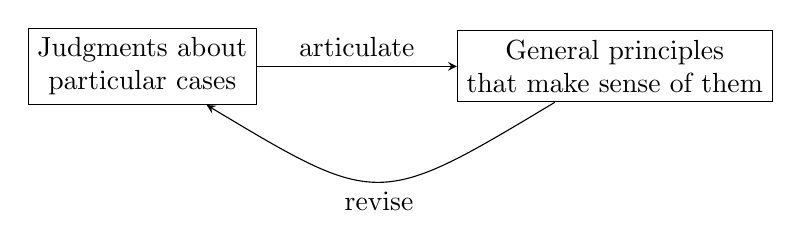
\begin{tikzpicture}[>=stealth]
\node[draw, rectangle, align=center] (A) at (0,0) {Judgments about\\particular cases};
\node[draw, rectangle, align=center] (B) at (6,0) {General principles\\that make sense of them};
\draw[->] (A) -- node[above] {articulate} (B);
\draw[->] (B) .. controls (3,-1.8) and (3,-1.8) .. node[below] {revise} (A);
\end{tikzpicture}
\end{figure}

We can set the procedure out explicitly:
\begin{enumerate}
\item We begin with considered judgments about cases, events, stories, and examples.
\item We formulate the principles that seem to explain those judgments.
\item We test whether the principles and judgments cohere.
\item When they do not, we revise our judgments, our principles, or both.
\end{enumerate}

Sandel then turns this method back on Rawls. Rawls accepts reflective equilibrium for questions of justice but not for comprehensive moral and religious questions. The reason, Rawls says, is the fact of reasonable pluralism: conscientious people who reason well may continue to disagree about the good life.

Sandel does not deny this fact. He presses instead on the boundary Rawls draws. Why should reasonable pluralism count as an obstacle in one domain but not in the other? We also disagree, and sometimes reasonably disagree, about justice itself. We disagree about liberty, equality, free markets, redistribution, free speech, and religious liberty. If reflective equilibrium remains our method in the case of justice despite such disagreement, why should the existence of disagreement bar its use when questions of the good are at stake?

This is the lecture's final philosophical reversal. Sandel is not simply turning Rawls into Aristotle. He is asking why the method Rawls accepts for one domain should be denied to the other when both domains exhibit deep, and sometimes reasonable, pluralism.

\section{Respect, Moral Engagement, and the Restlessness of Reason}

The final movement of the lecture addresses a liberal worry. If our disagreements about justice are bound up with disagreements about morality and religion, how can democratic life sustain mutual respect? Sandel's answer is that the worry depends on what we mean by respect.

One conception is the familiar liberal one:
\begin{equation}
\text{respect}_{\mathrm{liberal}}
=
\text{bracketing or abstracting from moral and religious convictions}.
\end{equation}
On this view, we respect our fellow citizens by setting their deeper moral and religious commitments aside for political purposes. We do not deny those commitments; we simply refrain from bringing them into public argument.

Sandel contrasts this with a more engaged conception:
\begin{equation}
\text{respect}_{\mathrm{engaged}}
=
\text{attending to, contesting, and learning from those convictions}.
\end{equation}
Here respect does not mean indifference. It means taking one another's convictions seriously enough to address them, sometimes by challenge, sometimes by listening, sometimes by genuine learning.

\subsection{Question \& Answer}

\paragraph{Question.} Does respect require setting moral convictions aside, or taking them seriously enough to engage them?

\paragraph{Answer.} Sandel argues for the second view. A politics of engagement offers no guarantee of agreement, and not even a guarantee of appreciation. We may come to understand a doctrine better and like it less. But for a pluralist society this model is, in his view, more honest and more adequate than a politics of abstraction.

The final conclusion is therefore not a final verdict on one controversy. It is a more general civic claim:
\begin{equation}
\text{politics of moral engagement}
\Longrightarrow
\text{better appreciation of plural human goods}.
\end{equation}
To the extent that our moral and religious disagreements reflect an irreducible plurality of human goods, a politics of moral engagement is better suited than a politics of bracketing to appreciating what different forms of life express.

The lecture then returns to the course's opening theme. Philosophy estranges us from the familiar. It unsettles settled assumptions. Once the familiar turns strange, it is never again simply what it was. Sandel's closing cadence is valedictory, but it remains argumentative. The persistence of these questions is not a defect of philosophy. It is the mark of its necessity. We live some answer to them all the time, in public life and in our personal lives.

This is why the lecture ends with Kant's image of the restlessness of reason. Skepticism may be a resting place, but it is no permanent dwelling place. The aim of the course has been to awaken that restlessness and to see where it might lead.

\section{Summary}

The lecture begins by reopening the argument over the narrative self and the reality of obligations of solidarity. It then tests the universalist challenge by asking what becomes of friendship if universal human concern must always override particular loyalties. From there Sandel sharpens the central philosophical issue: justice may be tied to the good in a relativist way or in a non-relativist way, and only the latter can preserve justice's critical force.

The lecture's middle movement uses same-sex marriage as a deliberately chosen stress test for neutrality. The classroom discussion generates the conceptual distinctions on which the chapter turns: procreation versus union, moral permissibility versus public recognition, neutrality versus disestablishment. Goodridge then shows at the institutional level what the classroom discussion had already begun to reveal: once the state remains in the business of honoring marriage, it cannot avoid reasoning about marriage's telos.

The final movement turns from inevitability to possibility. Reflective equilibrium supplies a model of moral reasoning that does not depend on a single master principle, and Sandel uses Rawls to show that disagreement does not by itself end public reasoning. The lecture closes with a substantive conception of respect. On Sandel's view, democratic respect is not best expressed by bracketing moral conviction, but by engaging it. The course therefore ends where it began: with philosophy as the unsettling of settled assumptions and with the restlessness of reason as a permanent feature of our common life.